\documentclass[a4paper,12pt]{article}

\usepackage{Packages}
\usepackage{subfigure}
\usepackage{amsmath}


\begin{document}
\begin{titlepage}

\begin{center}

% Upper part of the page. The '~' is needed because \\
% only works if a paragraph has started.

\includegraphics[width=0.6\textwidth]{./Figures/TUe}~\\[2cm]


%\vspace*{10cm}

% Title
\HRule \\[0.4cm]
{ \huge \bfseries 2IMM20 - Foundations of datamining\\[0.3cm] }
\HRule \\[1.5cm]
\textbf{Assignment 2}


% Author and supervisor

\vfill

\begin{table}[h]
\begin{tabular}{ll}
\textbf{Students:} & \\
Joris van der Heijden & (0937329)\\
Bram van der Pol & (0780042)\\

\\
\textbf{Email addresseses:} & \\
j.j.m.v.d.heijden@student.tue.nl \\
a.f.v.d.pol@student.tue.nl \\
\\
\textbf{Supervisors:} &\\
Dr.ir. Joaquin Vanschoren
\\

%\textbf{Supervisors:} & \\
%Dr. M.Holenderski \\
\end{tabular}
\end{table}



% Bottom of the page
\large
{ Eindhoven, \today}

\end{center}


\end{titlepage}
 %included in part 1

\tableofcontents %included in part 1

\section*{Nepalese character recognition}
\subsection*{1}
{\it Evaluate k-Nearest Neighbors, Logistic Regression and RandomForests with their default
settings.
\begin{itemize}
\item{Take a stratified 10\% subsample of the data.}
\item{Use the default train-test split and predictive accuracy. Is predictive accuracy a good scoring measure for this problem?}
\item{Try to build the same models on increasingly large samples of the dataset (e.g. 10\%,
20\%,...). Plot the training time and the predictive performance for each. Stop when the
training time becomes prohibitively large (this will be different for different models).}
\end{itemize}
\textnormal{Because the logistic regression algorithm took more time than the k-Nearest and the Random Forest algorithm we made two figures; one based on maximum 20\% of the data and one based on maximum 6\% of the data. For this problem we used 75\% of the data to train the model and 25\% to validate the model.}

\begin{figure}[H]
\hfill
\makebox[\textwidth][c]{{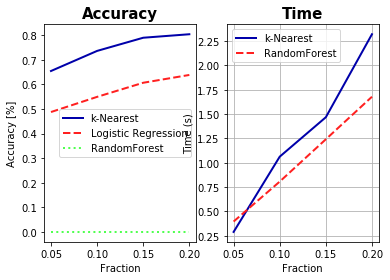
\includegraphics[width=12cm]{./Figures/output_15_1}}}
\hfill
\caption{Performance of the k-Nearest and Logistic regression algorithms. }
\label{Q21a}
\end{figure}

\begin{figure}[H]
\hfill
\makebox[\textwidth][c]{{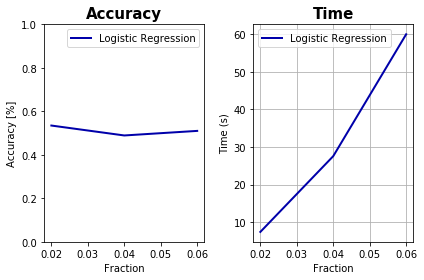
\includegraphics[width=12cm]{./Figures/output_15_3}}}
\hfill
\caption{Performance of the Logistic regression algorithm.}
\label{Q21b}
\end{figure}

\textnormal{Because the data size is sufficiently large the predictive accuracy is a good scoring measure. The characteristics of the k-Nearest and randomForest algorithm is shown in figure \ref{Q21a}. This figures shows that the accuracy of the models goes up when more data is used, which is expected. However figure \ref{Q21b} does not show this trend. We do not recommend this algorithm for this problem because of the time needed to train this algorithm and the accuracy of the model.}


\subsection*{2}
{\it Optimize the value for the number of neighbors $k$ (keep $k < 50$) and the number of trees
(keep $n_{estimators} < 100$) on the stratified 10\% subsample. Use 10-fold crossvalidation and plot $k$ and $n_{estimators}$ against the predictive accuracy. Which value of $k, n_{estimators}$ should you pick?}\\

\begin{figure}[H]
\hfill
\makebox[\textwidth][c]{
\subfigure[]{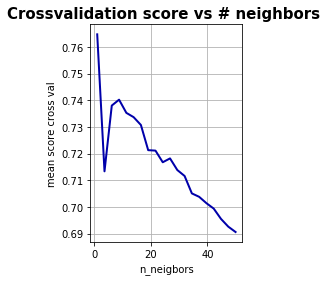
\includegraphics[width=6cm]{./Figures/output_17_1}}
\subfigure[]{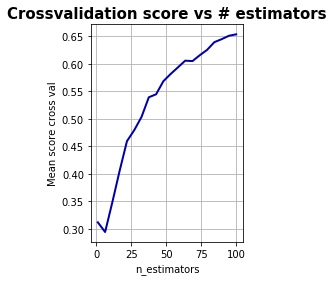
\includegraphics[width=6cm]{./Figures/output_17_3}}}
\hfill
\caption{}
\label{Q22}
\end{figure}
As can been seen in figure \ref{Q22} is that the number of neigbors should be set to 1 and the number of trees to 100. 

\subsection*{3}
{\it For the RandomForest, optimize both $n_{estimators}$ and $max_{features}$ at the same time on the entire dataset. - Use a nested cross-validation and a random search over the possible values, and measure the accuracy. Explore how fine-grained this grid/random search can be, given your computational resources. What is the optimal performance you find? - Hint: choose a nested cross-validation that is feasible. Don’t use too many folds in the outer loop. - Repeat the grid search and visualize the results as a plot (heatmap) $n_{estimators}\cdot max_{features} \rightarrow ACC$ with ACC visualized as the color of the data point. Try to make the grid as fine as possible. Interpret the results. Can you explain your observations? What did you learn about tuning RandomForests?}
\begin{figure}[H]
\hfill
\makebox[\textwidth][c]{{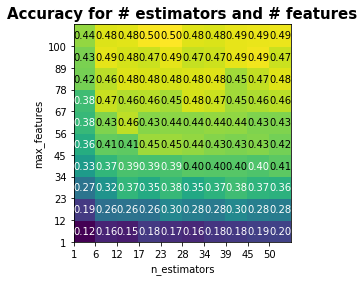
\includegraphics[width=12cm]{./Figures/output_19_1}}}
\hfill
\caption{Accuracy for the random forest for different maximum features and number of estimators numbers. This is done for 1\% of the total data set (due to the lack of computer power and time).}
\label{Q23}
\end{figure}
\textnormal{The finest grid which does not take too much time is in our case a 10x10 grid. This grid gives a good insight in the performance of the randomforest algorithm. We used only 1\% of the data because, unfortunately, the computing time was very large for 10\% of the data. This has a big influences on the results, however the characteristics of the algorithm can be examined. Figure \ref{Q23} shows that the number of trees in the forest. The optimal performance can be achieved by setting the number of estimators between 17 and 23 and the maximum features to 100. The more features that are available the better the data can be fitted, however overfitting the data can become a problem when the maximum number of features increases. The best number of trees does show a good accuracy for 50 number of trees. However the best accuracy can be increased by tuning the number of trees for a specific number of features.} 

\section*{4}
\subsection{1}
{\it Do a bias-variance analysis of both algorithms. For each, vary the number of trees on a log scale from 1 to 1024, and plot the bias error (squared), variance, and total error (in one plot per algorithm). Interpret the results. Which error is highest for small ensembles, and which reduced most by each algorithm as you use a larger ensemble? When are both algorithms under- or over-fitting? Provide a detailed explanation of why random forests and gradient boosting behave this way. - See lecture 3 for an example on how to do the bias-variance decomposition - To save time, you can use a 10\% stratified subsample in your initial experiments, but show the plots for the full dataset in your report. In [ ]: from sklearn.model}

\begin{figure}[H]
\hfill
\makebox[\textwidth][c]{{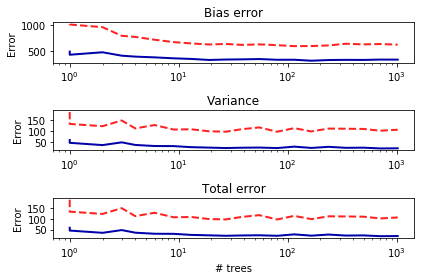
\includegraphics[width=12cm]{./Figures/output_24_1}}}
\hfill
\caption{RandomForests (blue lines )and Gradient Boosting (red dashed lines) as a function of the number of trees/ iterations.}
\label{Q41}
\end{figure}

\textnormal{The results shown in figure \ref{Q41} are not the results we expected. %We expected that the RandomForests and Gradient Boosting lines cross each other when the number of trees increases. This due to  
In general when the number of features/ iterations increased the model tend to overfit the data. However in this case each features is a pixel and the data is not overfitted. This also means that when the number of trees/ iterations increases all bias, variance and total errors goes down for this example. At the start both models are clearly under fitting because the number of total features of the image (1024) cannot be captured well. }

\subsection{2}
{\it A validation curve can help you understand when a model starts under- or overfitting. It plots both training and test set error as you change certain characteristics of your model, e.g. one or more hyperparameters. Build validation curves for gradient boosting, evaluated using AUROC, by varying the number of iterations between 1 and 500. In addition, use at least two values for the learning rate (e.g. 0.1 and 1), and tree depth (e.g. 1 and 4). This will yield at least 4 curves. Interpret the results and provide a clear explanation for the results. When is the model over- or underfitting? Discuss the effect of the different combinations learning rate and tree depth and provide a clear explanation.
While scikit-learn has a validation curve function, we'll use a modified version (below) that provides a lot more detail and can be used to study more than one hyperparameter. You can use a default train-test split.}

\textnormal{We added the $clf.fit(X\; train,y\; train)$ function before the Gradient boosting algorithm in order to make sere estimator was defined. The result is shown in figure \ref{Q41a} and figure \ref{Q41b}.}
 
\begin{figure}[H]
\hfill
\makebox[\textwidth][c]{{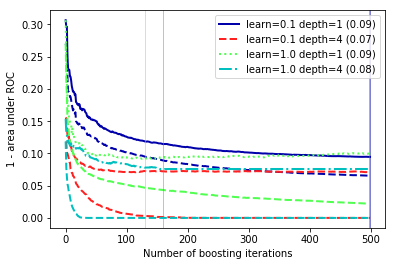
\includegraphics[width=12cm]{./Figures/output_26_3}}}
\hfill
\caption{Compute Receiver operating characteristic score for different hyperparameters for the gradient boosting algorithm.}
\label{Q41a}
\end{figure}
Figure \ref{Q41a} clearly shows the underfitting when the number of boosting iterations are small. The convergence rate for the learning rate of 1 is clearly faster than for 0.1. The tree depth also has a big influence on the convergence rate, see the light blue and red lines. More features can be captured in the model so the model can captures the model more accurately. The expected overfitting of the data (the increase of the 1-ROC value) does not happen for 500 iterations so therefore we made an example for 5000 iterations, figure \ref{Q41b}. 
\begin{figure}[H]
\hfill
\makebox[\textwidth][c]{{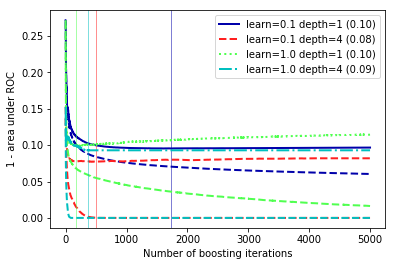
\includegraphics[width=12cm]{./Figures/output_26_2}}}
\hfill
\caption{Compute Receiver operating characteristic score for different hyperparameters for the gradient boosting algorithm. The number of iterations is set to 5000 to show possible overfitting characteristics.}
\label{Q41b}
\end{figure}
Overfitting of the data is not clearly visible even for 5000 iterations. 

\section{Appendix}
\subsection{Code question 2.1}
\label{AQ21}


\subsection{Code question 2.2}



\end{document}
